\documentclass[1p]{elsarticle_modified}
%\bibliographystyle{elsarticle-num}

%\usepackage[colorlinks]{hyperref}
%\usepackage{abbrmath_seonhwa} %\Abb, \Ascr, \Acal ,\Abf, \Afrak
\usepackage{amsfonts}
\usepackage{amssymb}
\usepackage{amsmath}
\usepackage{amsthm}
\usepackage{scalefnt}
\usepackage{amsbsy}
\usepackage{kotex}
\usepackage{caption}
\usepackage{subfig}
\usepackage{color}
\usepackage{graphicx}
\usepackage{xcolor} %% white, black, red, green, blue, cyan, magenta, yellow
\usepackage{float}
\usepackage{setspace}
\usepackage{hyperref}

\usepackage{tikz}
\usetikzlibrary{arrows}

\usepackage{multirow}
\usepackage{array} % fixed length table
\usepackage{hhline}

%%%%%%%%%%%%%%%%%%%%%
\makeatletter
\renewcommand*\env@matrix[1][\arraystretch]{%
	\edef\arraystretch{#1}%
	\hskip -\arraycolsep
	\let\@ifnextchar\new@ifnextchar
	\array{*\c@MaxMatrixCols c}}
\makeatother %https://tex.stackexchange.com/questions/14071/how-can-i-increase-the-line-spacing-in-a-matrix
%%%%%%%%%%%%%%%

\usepackage[normalem]{ulem}

\newcommand{\msout}[1]{\ifmmode\text{\sout{\ensuremath{#1}}}\else\sout{#1}\fi}
%SOURCE: \msout is \stkout macro in https://tex.stackexchange.com/questions/20609/strikeout-in-math-mode

\newcommand{\cancel}[1]{
	\ifmmode
	{\color{red}\msout{#1}}
	\else
	{\color{red}\sout{#1}}
	\fi
}

\newcommand{\add}[1]{
	{\color{blue}\uwave{#1}}
}

\newcommand{\replace}[2]{
	\ifmmode
	{\color{red}\msout{#1}}{\color{blue}\uwave{#2}}
	\else
	{\color{red}\sout{#1}}{\color{blue}\uwave{#2}}
	\fi
}

\newcommand{\Sol}{\mathcal{S}} %segment
\newcommand{\D}{D} %diagram
\newcommand{\A}{\mathcal{A}} %arc


%%%%%%%%%%%%%%%%%%%%%%%%%%%%%5 test

\def\sl{\operatorname{\textup{SL}}(2,\Cbb)}
\def\psl{\operatorname{\textup{PSL}}(2,\Cbb)}
\def\quan{\mkern 1mu \triangleright \mkern 1mu}

\theoremstyle{definition}
\newtheorem{thm}{Theorem}[section]
\newtheorem{prop}[thm]{Proposition}
\newtheorem{lem}[thm]{Lemma}
\newtheorem{ques}[thm]{Question}
\newtheorem{cor}[thm]{Corollary}
\newtheorem{defn}[thm]{Definition}
\newtheorem{exam}[thm]{Example}
\newtheorem{rmk}[thm]{Remark}
\newtheorem{alg}[thm]{Algorithm}

\newcommand{\I}{\sqrt{-1}}
\begin{document}

%\begin{frontmatter}
%
%\title{Boundary parabolic representations of knots up to 8 crossings}
%
%%% Group authors per affiliation:
%\author{Yunhi Cho} 
%\address{Department of Mathematics, University of Seoul, Seoul, Korea}
%\ead{yhcho@uos.ac.kr}
%
%
%\author{Seonhwa Kim} %\fnref{s_kim}}
%\address{Center for Geometry and Physics, Institute for Basic Science, Pohang, 37673, Korea}
%\ead{ryeona17@ibs.re.kr}
%
%\author{Hyuk Kim}
%\address{Department of Mathematical Sciences, Seoul National University, Seoul 08826, Korea}
%\ead{hyukkim@snu.ac.kr}
%
%\author{Seokbeom Yoon}
%\address{Department of Mathematical Sciences, Seoul National University, Seoul, 08826,  Korea}
%\ead{sbyoon15@snu.ac.kr}
%
%\begin{abstract}
%We find all boundary parabolic representation of knots up to 8 crossings.
%
%\end{abstract}
%\begin{keyword}
%    \MSC[2010] 57M25 
%\end{keyword}
%
%\end{frontmatter}

%\linenumbers
%\tableofcontents
%
\newcommand\colored[1]{\textcolor{white}{\rule[-0.35ex]{0.8em}{1.4ex}}\kern-0.8em\color{red} #1}%
%\newcommand\colored[1]{\textcolor{white}{ #1}\kern-2.17ex	\textcolor{white}{ #1}\kern-1.81ex	\textcolor{white}{ #1}\kern-2.15ex\color{red}#1	}

{\Large $\underline{12a_{0585}~(K12a_{0585})}$}

\setlength{\tabcolsep}{10pt}
\renewcommand{\arraystretch}{1.6}
\vspace{1cm}\begin{tabular}{m{100pt}>{\centering\arraybackslash}m{274pt}}
\multirow{5}{120pt}{
	\centering
	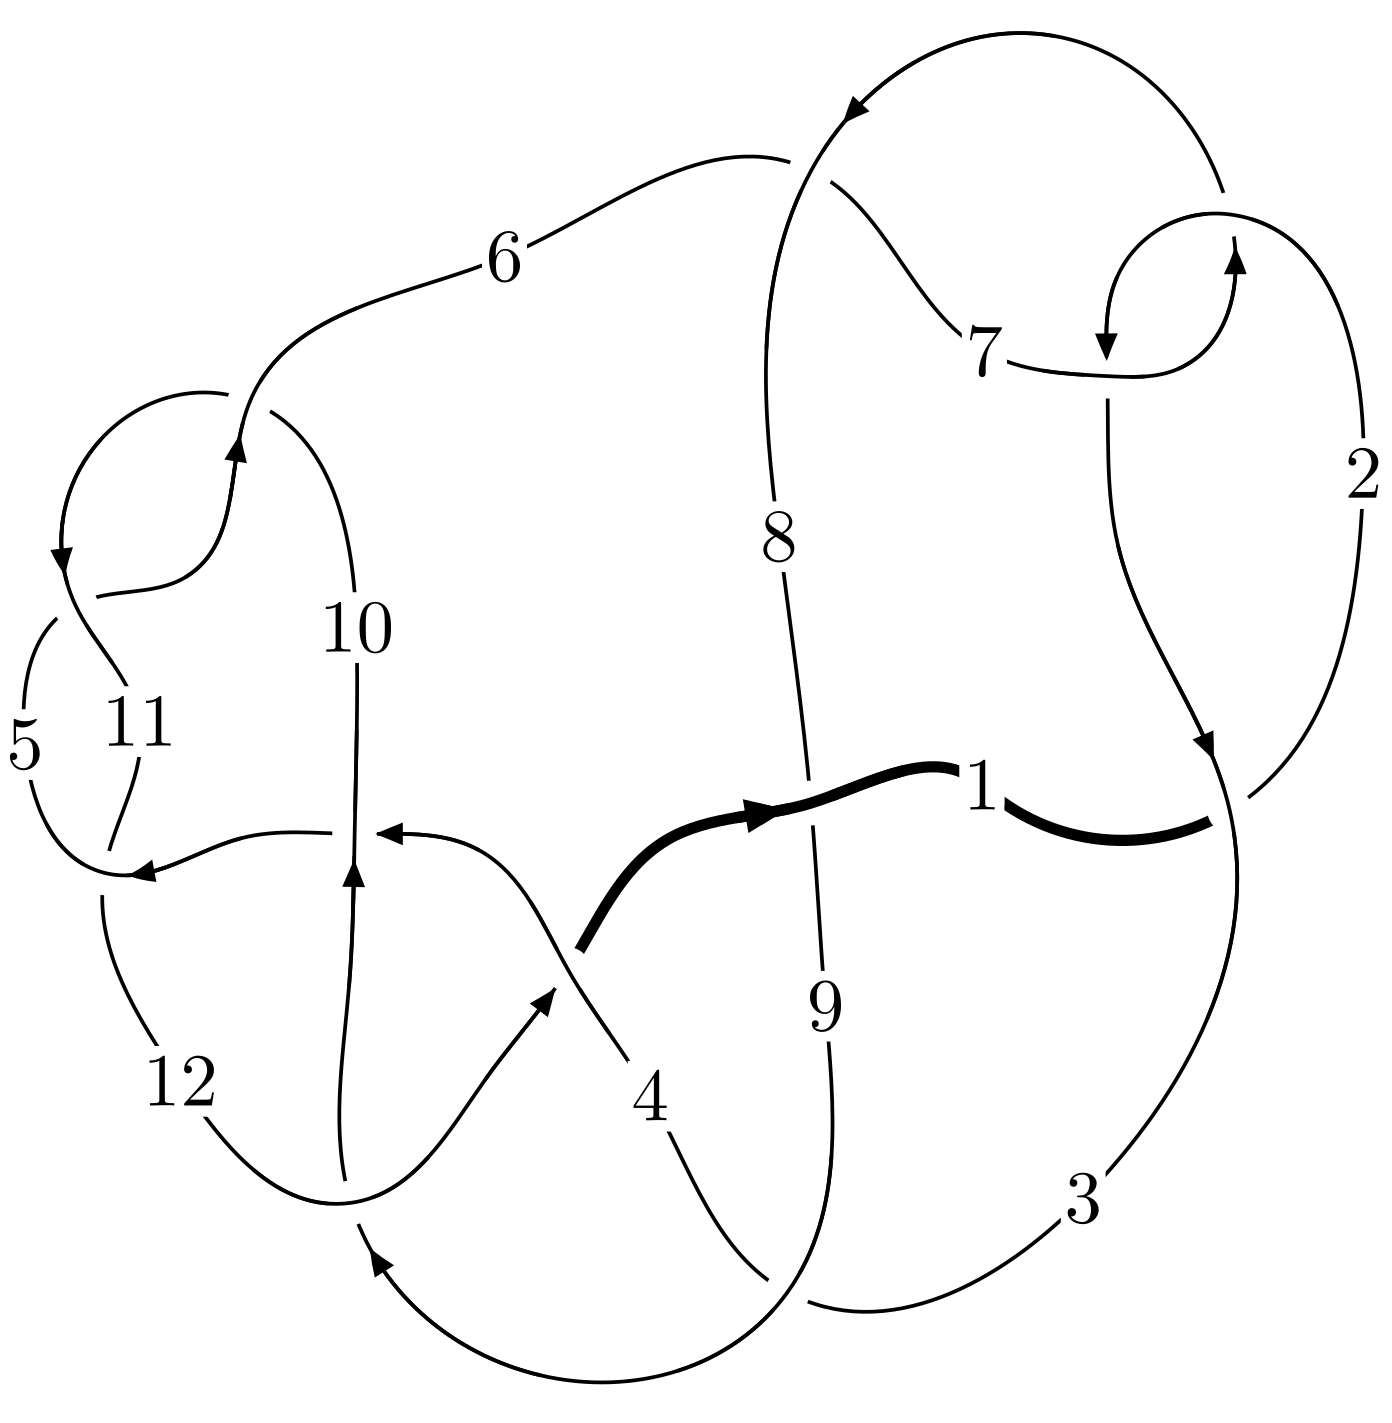
\includegraphics[width=112pt]{../../../GIT/diagram.site/Diagrams/png/1386_12a_0585.png}\\
\ \ \ A knot diagram\footnotemark}&
\allowdisplaybreaks
\textbf{Linearized knot diagam} \\
\cline{2-2}
 &
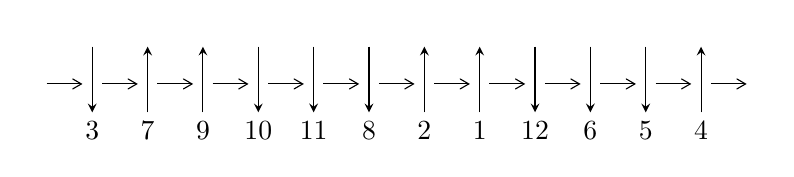
\begin{tikzpicture}[x=20pt, y=17pt]
	% nodes
	\node (C0) at (0, 0) {};
	\node (C1) at (1, 0) {};
	\node (C1U) at (1, +1) {};
	\node (C1D) at (1, -1) {3};

	\node (C2) at (2, 0) {};
	\node (C2U) at (2, +1) {};
	\node (C2D) at (2, -1) {7};

	\node (C3) at (3, 0) {};
	\node (C3U) at (3, +1) {};
	\node (C3D) at (3, -1) {9};

	\node (C4) at (4, 0) {};
	\node (C4U) at (4, +1) {};
	\node (C4D) at (4, -1) {10};

	\node (C5) at (5, 0) {};
	\node (C5U) at (5, +1) {};
	\node (C5D) at (5, -1) {11};

	\node (C6) at (6, 0) {};
	\node (C6U) at (6, +1) {};
	\node (C6D) at (6, -1) {8};

	\node (C7) at (7, 0) {};
	\node (C7U) at (7, +1) {};
	\node (C7D) at (7, -1) {2};

	\node (C8) at (8, 0) {};
	\node (C8U) at (8, +1) {};
	\node (C8D) at (8, -1) {1};

	\node (C9) at (9, 0) {};
	\node (C9U) at (9, +1) {};
	\node (C9D) at (9, -1) {12};

	\node (C10) at (10, 0) {};
	\node (C10U) at (10, +1) {};
	\node (C10D) at (10, -1) {6};

	\node (C11) at (11, 0) {};
	\node (C11U) at (11, +1) {};
	\node (C11D) at (11, -1) {5};

	\node (C12) at (12, 0) {};
	\node (C12U) at (12, +1) {};
	\node (C12D) at (12, -1) {4};
	\node (C13) at (13, 0) {};

	% arrows
	\draw[->,>={angle 60}]
	(C0) edge (C1) (C1) edge (C2) (C2) edge (C3) (C3) edge (C4) (C4) edge (C5) (C5) edge (C6) (C6) edge (C7) (C7) edge (C8) (C8) edge (C9) (C9) edge (C10) (C10) edge (C11) (C11) edge (C12) (C12) edge (C13) ;	\draw[->,>=stealth]
	(C1U) edge (C1D) (C2D) edge (C2U) (C3D) edge (C3U) (C4U) edge (C4D) (C5U) edge (C5D) (C6U) edge (C6D) (C7D) edge (C7U) (C8D) edge (C8U) (C9U) edge (C9D) (C10U) edge (C10D) (C11U) edge (C11D) (C12D) edge (C12U) ;
	\end{tikzpicture} \\
\hhline{~~} \\& 
\textbf{Solving Sequence} \\ \cline{2-2} 
 &
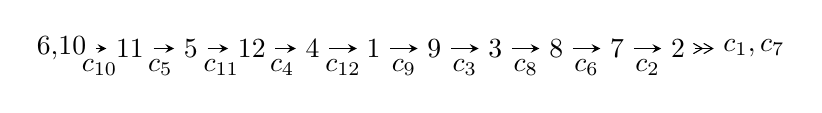
\begin{tikzpicture}[x=22pt, y=7pt]
	% node
	\node (A0) at (-1/8, 0) {6,10};
	\node (A1) at (1, 0) {11};
	\node (A2) at (2, 0) {5};
	\node (A3) at (3, 0) {12};
	\node (A4) at (4, 0) {4};
	\node (A5) at (5, 0) {1};
	\node (A6) at (6, 0) {9};
	\node (A7) at (7, 0) {3};
	\node (A8) at (8, 0) {8};
	\node (A9) at (9, 0) {7};
	\node (A10) at (10, 0) {2};
	\node (C1) at (1/2, -1) {$c_{10}$};
	\node (C2) at (3/2, -1) {$c_{5}$};
	\node (C3) at (5/2, -1) {$c_{11}$};
	\node (C4) at (7/2, -1) {$c_{4}$};
	\node (C5) at (9/2, -1) {$c_{12}$};
	\node (C6) at (11/2, -1) {$c_{9}$};
	\node (C7) at (13/2, -1) {$c_{3}$};
	\node (C8) at (15/2, -1) {$c_{8}$};
	\node (C9) at (17/2, -1) {$c_{6}$};
	\node (C10) at (19/2, -1) {$c_{2}$};
	\node (A11) at (45/4, 0) {$c_{1},c_{7}$};

	% edge
	\draw[->,>=stealth]	
	(A0) edge (A1) (A1) edge (A2) (A2) edge (A3) (A3) edge (A4) (A4) edge (A5) (A5) edge (A6) (A6) edge (A7) (A7) edge (A8) (A8) edge (A9) (A9) edge (A10) ;
	\draw[->>,>={angle 60}]	
	(A10) edge (A11);
\end{tikzpicture} \\ 

\end{tabular} \\

\footnotetext{
The image of knot diagram is generated by the software ``\textbf{Draw programme}" developed by Andrew Bartholomew(\url{http://www.layer8.co.uk/maths/draw/index.htm\#Running-draw}), where we modified some parts for our purpose(\url{https://github.com/CATsTAILs/LinksPainter}).
}\phantom \\ \newline 
\centering \textbf{Ideals for irreducible components\footnotemark of $X_{\text{par}}$} 
 
\begin{align*}
I^u_{1}&=\langle 
u^{90}- u^{89}+\cdots-3 u+1\rangle \\
\\
\end{align*}
\raggedright * 1 irreducible components of $\dim_{\mathbb{C}}=0$, with total 90 representations.\\
\footnotetext{All coefficients of polynomials are rational numbers. But the coefficients are sometimes approximated in decimal forms when there is not enough margin.}
\newpage
\renewcommand{\arraystretch}{1}
\centering \section*{I. $I^u_{1}= \langle u^{90}- u^{89}+\cdots-3 u+1 \rangle$}
\flushleft \textbf{(i) Arc colorings}\\
\begin{tabular}{m{7pt} m{180pt} m{7pt} m{180pt} }
\flushright $a_{6}=$&$\begin{pmatrix}0\\u\end{pmatrix}$ \\
\flushright $a_{10}=$&$\begin{pmatrix}1\\0\end{pmatrix}$ \\
\flushright $a_{11}=$&$\begin{pmatrix}1\\u^2\end{pmatrix}$ \\
\flushright $a_{5}=$&$\begin{pmatrix}u\\u^3+u\end{pmatrix}$ \\
\flushright $a_{12}=$&$\begin{pmatrix}u^2+1\\u^4+2 u^2\end{pmatrix}$ \\
\flushright $a_{4}=$&$\begin{pmatrix}u^3+2 u\\u^3+u\end{pmatrix}$ \\
\flushright $a_{1}=$&$\begin{pmatrix}u^{10}+5 u^8+8 u^6+3 u^4- u^2+1\\u^{10}+4 u^8+5 u^6+2 u^4+u^2\end{pmatrix}$ \\
\flushright $a_{9}=$&$\begin{pmatrix}- u^6-3 u^4-2 u^2+1\\- u^8-4 u^6-4 u^4\end{pmatrix}$ \\
\flushright $a_{3}=$&$\begin{pmatrix}u^{17}+8 u^{15}+25 u^{13}+36 u^{11}+19 u^9-4 u^7-2 u^5+4 u^3+u\\u^{19}+9 u^{17}+32 u^{15}+55 u^{13}+43 u^{11}+9 u^9+4 u^5+u^3+u\end{pmatrix}$ \\
\flushright $a_{8}=$&$\begin{pmatrix}u^{28}+13 u^{26}+\cdots- u^2+1\\u^{28}+12 u^{26}+\cdots+2 u^6-3 u^4\end{pmatrix}$ \\
\flushright $a_{7}=$&$\begin{pmatrix}- u^{57}-26 u^{55}+\cdots+2 u^3- u\\- u^{57}-25 u^{55}+\cdots+3 u^5+u\end{pmatrix}$ \\
\flushright $a_{2}=$&$\begin{pmatrix}u^{46}+21 u^{44}+\cdots+6 u^4+1\\u^{48}+22 u^{46}+\cdots+2 u^4+2 u^2\end{pmatrix}$\\&\end{tabular}
\flushleft \textbf{(ii) Obstruction class $= -1$}\\~\\
\flushleft \textbf{(iii) Cusp Shapes $= 4 u^{89}-4 u^{88}+\cdots+20 u-10$}\\~\\
\newpage\renewcommand{\arraystretch}{1}
\flushleft \textbf{(iv) u-Polynomials at the component}\newline \\
\begin{tabular}{m{50pt}|m{274pt}}
Crossings & \hspace{64pt}u-Polynomials at each crossing \\
\hline $$\begin{aligned}c_{1},c_{6}\end{aligned}$$&$\begin{aligned}
&u^{90}+29 u^{89}+\cdots+u+1
\end{aligned}$\\
\hline $$\begin{aligned}c_{2},c_{7}\end{aligned}$$&$\begin{aligned}
&u^{90}+u^{89}+\cdots- u+1
\end{aligned}$\\
\hline $$\begin{aligned}c_{3}\end{aligned}$$&$\begin{aligned}
&u^{90}+u^{89}+\cdots+5329 u+2941
\end{aligned}$\\
\hline $$\begin{aligned}c_{4}\end{aligned}$$&$\begin{aligned}
&u^{90}- u^{89}+\cdots+11 u+1
\end{aligned}$\\
\hline $$\begin{aligned}c_{5},c_{10},c_{11}\end{aligned}$$&$\begin{aligned}
&u^{90}+u^{89}+\cdots+3 u+1
\end{aligned}$\\
\hline $$\begin{aligned}c_{8}\end{aligned}$$&$\begin{aligned}
&u^{90}-5 u^{89}+\cdots- u+1
\end{aligned}$\\
\hline $$\begin{aligned}c_{9}\end{aligned}$$&$\begin{aligned}
&u^{90}-19 u^{89}+\cdots-88451 u+4523
\end{aligned}$\\
\hline $$\begin{aligned}c_{12}\end{aligned}$$&$\begin{aligned}
&u^{90}+7 u^{89}+\cdots+941 u+55
\end{aligned}$\\
\hline
\end{tabular}\\~\\
\newpage\renewcommand{\arraystretch}{1}
\flushleft \textbf{(v) Riley Polynomials at the component}\newline \\
\begin{tabular}{m{50pt}|m{274pt}}
Crossings & \hspace{64pt}Riley Polynomials at each crossing \\
\hline $$\begin{aligned}c_{1},c_{6}\end{aligned}$$&$\begin{aligned}
&y^{90}+65 y^{89}+\cdots+5 y+1
\end{aligned}$\\
\hline $$\begin{aligned}c_{2},c_{7}\end{aligned}$$&$\begin{aligned}
&y^{90}+29 y^{89}+\cdots+y+1
\end{aligned}$\\
\hline $$\begin{aligned}c_{3}\end{aligned}$$&$\begin{aligned}
&y^{90}-27 y^{89}+\cdots-251343687 y+8649481
\end{aligned}$\\
\hline $$\begin{aligned}c_{4}\end{aligned}$$&$\begin{aligned}
&y^{90}+5 y^{89}+\cdots-47 y+1
\end{aligned}$\\
\hline $$\begin{aligned}c_{5},c_{10},c_{11}\end{aligned}$$&$\begin{aligned}
&y^{90}+81 y^{89}+\cdots+y+1
\end{aligned}$\\
\hline $$\begin{aligned}c_{8}\end{aligned}$$&$\begin{aligned}
&y^{90}+y^{89}+\cdots+29 y+1
\end{aligned}$\\
\hline $$\begin{aligned}c_{9}\end{aligned}$$&$\begin{aligned}
&y^{90}+29 y^{89}+\cdots+330837793 y+20457529
\end{aligned}$\\
\hline $$\begin{aligned}c_{12}\end{aligned}$$&$\begin{aligned}
&y^{90}+13 y^{89}+\cdots+155009 y+3025
\end{aligned}$\\
\hline
\end{tabular}\\~\\
\newpage\flushleft \textbf{(vi) Complex Volumes and Cusp Shapes}
$$\begin{array}{c|c|c}  
\text{Solutions to }I^u_{1}& \I (\text{vol} + \sqrt{-1}CS) & \text{Cusp shape}\\
 \hline 
\begin{aligned}
u &= -0.092360 + 0.990486 I\end{aligned}
 & -0.19734 - 2.09371 I & \phantom{-0.000000 } 0 \\ \hline\begin{aligned}
u &= -0.092360 - 0.990486 I\end{aligned}
 & -0.19734 + 2.09371 I & \phantom{-0.000000 } 0 \\ \hline\begin{aligned}
u &= -0.174167 + 1.065840 I\end{aligned}
 & -2.74452 + 3.55694 I & \phantom{-0.000000 } 0 \\ \hline\begin{aligned}
u &= -0.174167 - 1.065840 I\end{aligned}
 & -2.74452 - 3.55694 I & \phantom{-0.000000 } 0 \\ \hline\begin{aligned}
u &= \phantom{-}0.109638 + 1.103100 I\end{aligned}
 & \phantom{-}1.18483 - 1.77466 I & \phantom{-0.000000 } 0 \\ \hline\begin{aligned}
u &= \phantom{-}0.109638 - 1.103100 I\end{aligned}
 & \phantom{-}1.18483 + 1.77466 I & \phantom{-0.000000 } 0 \\ \hline\begin{aligned}
u &= -0.208911 + 1.105270 I\end{aligned}
 & \phantom{-}2.33069 + 9.15031 I & \phantom{-0.000000 } 0 \\ \hline\begin{aligned}
u &= -0.208911 - 1.105270 I\end{aligned}
 & \phantom{-}2.33069 - 9.15031 I & \phantom{-0.000000 } 0 \\ \hline\begin{aligned}
u &= \phantom{-}0.196314 + 1.116870 I\end{aligned}
 & \phantom{-}3.28147 - 3.51353 I & \phantom{-0.000000 } 0 \\ \hline\begin{aligned}
u &= \phantom{-}0.196314 - 1.116870 I\end{aligned}
 & \phantom{-}3.28147 + 3.51353 I & \phantom{-0.000000 } 0 \\ \hline\begin{aligned}
u &= \phantom{-}0.708793 + 0.299494 I\end{aligned}
 & \phantom{-}1.68759 - 12.58900 I & -1.92424 + 10.40743 I \\ \hline\begin{aligned}
u &= \phantom{-}0.708793 - 0.299494 I\end{aligned}
 & \phantom{-}1.68759 + 12.58900 I & -1.92424 - 10.40743 I \\ \hline\begin{aligned}
u &= -0.703274 + 0.301535 I\end{aligned}
 & \phantom{-}2.64941 + 6.81481 I & -0.10297 - 5.63570 I \\ \hline\begin{aligned}
u &= -0.703274 - 0.301535 I\end{aligned}
 & \phantom{-}2.64941 - 6.81481 I & -0.10297 + 5.63570 I \\ \hline\begin{aligned}
u &= \phantom{-}0.700545 + 0.282219 I\end{aligned}
 & -3.78579 - 6.94246 I & -7.67165 + 8.00926 I \\ \hline\begin{aligned}
u &= \phantom{-}0.700545 - 0.282219 I\end{aligned}
 & -3.78579 + 6.94246 I & -7.67165 - 8.00926 I \\ \hline\begin{aligned}
u &= -0.678301 + 0.287933 I\end{aligned}
 & \phantom{-}0.05334 + 4.69227 I & \phantom{-}0.02736 - 6.79114 I \\ \hline\begin{aligned}
u &= -0.678301 - 0.287933 I\end{aligned}
 & \phantom{-}0.05334 - 4.69227 I & \phantom{-}0.02736 + 6.79114 I \\ \hline\begin{aligned}
u &= \phantom{-}0.384609 + 0.625740 I\end{aligned}
 & \phantom{-}2.97480 + 8.70845 I & \phantom{-}0.78880 - 5.17975 I \\ \hline\begin{aligned}
u &= \phantom{-}0.384609 - 0.625740 I\end{aligned}
 & \phantom{-}2.97480 - 8.70845 I & \phantom{-}0.78880 + 5.17975 I \\ \hline\begin{aligned}
u &= -0.646374 + 0.328778 I\end{aligned}
 & \phantom{-}4.40452 + 4.07878 I & \phantom{-}2.14162 - 6.13926 I \\ \hline\begin{aligned}
u &= -0.646374 - 0.328778 I\end{aligned}
 & \phantom{-}4.40452 - 4.07878 I & \phantom{-}2.14162 + 6.13926 I \\ \hline\begin{aligned}
u &= \phantom{-}0.677349 + 0.249229 I\end{aligned}
 & -1.86025 - 1.15632 I & -5.97482 + 1.58422 I \\ \hline\begin{aligned}
u &= \phantom{-}0.677349 - 0.249229 I\end{aligned}
 & -1.86025 + 1.15632 I & -5.97482 - 1.58422 I \\ \hline\begin{aligned}
u &= -0.386229 + 0.609030 I\end{aligned}
 & \phantom{-}3.89211 - 2.96681 I & \phantom{-}2.65198 + 0.23669 I \\ \hline\begin{aligned}
u &= -0.386229 - 0.609030 I\end{aligned}
 & \phantom{-}3.89211 + 2.96681 I & \phantom{-}2.65198 - 0.23669 I \\ \hline\begin{aligned}
u &= \phantom{-}0.633442 + 0.335557 I\end{aligned}
 & \phantom{-}3.95811 + 1.65651 I & \phantom{-}1.36233 + 0.56944 I \\ \hline\begin{aligned}
u &= \phantom{-}0.633442 - 0.335557 I\end{aligned}
 & \phantom{-}3.95811 - 1.65651 I & \phantom{-}1.36233 - 0.56944 I \\ \hline\begin{aligned}
u &= -0.677616 + 0.197513 I\end{aligned}
 & -2.43312 + 5.36697 I & -7.06462 - 7.35684 I \\ \hline\begin{aligned}
u &= -0.677616 - 0.197513 I\end{aligned}
 & -2.43312 - 5.36697 I & -7.06462 + 7.35684 I\\
 \hline 
 \end{array}$$\newpage$$\begin{array}{c|c|c}  
\text{Solutions to }I^u_{1}& \I (\text{vol} + \sqrt{-1}CS) & \text{Cusp shape}\\
 \hline 
\begin{aligned}
u &= \phantom{-}0.031544 + 1.295490 I\end{aligned}
 & \phantom{-}5.21152 - 2.64980 I & \phantom{-0.000000 } 0 \\ \hline\begin{aligned}
u &= \phantom{-}0.031544 - 1.295490 I\end{aligned}
 & \phantom{-}5.21152 + 2.64980 I & \phantom{-0.000000 } 0 \\ \hline\begin{aligned}
u &= \phantom{-}0.322486 + 0.620173 I\end{aligned}
 & -2.39255 + 3.21804 I & -4.96336 - 2.89069 I \\ \hline\begin{aligned}
u &= \phantom{-}0.322486 - 0.620173 I\end{aligned}
 & -2.39255 - 3.21804 I & -4.96336 + 2.89069 I \\ \hline\begin{aligned}
u &= -0.669378 + 0.147993 I\end{aligned}
 & -5.42459 - 0.27478 I & -11.47130 - 0.26528 I \\ \hline\begin{aligned}
u &= -0.669378 - 0.147993 I\end{aligned}
 & -5.42459 + 0.27478 I & -11.47130 + 0.26528 I \\ \hline\begin{aligned}
u &= -0.673819 + 0.103290 I\end{aligned}
 & -0.64886 - 5.80042 I & -5.73200 + 4.09941 I \\ \hline\begin{aligned}
u &= -0.673819 - 0.103290 I\end{aligned}
 & -0.64886 + 5.80042 I & -5.73200 - 4.09941 I \\ \hline\begin{aligned}
u &= \phantom{-}0.472908 + 0.471039 I\end{aligned}
 & \phantom{-}4.58313 - 5.28881 I & \phantom{-}3.03353 + 6.59017 I \\ \hline\begin{aligned}
u &= \phantom{-}0.472908 - 0.471039 I\end{aligned}
 & \phantom{-}4.58313 + 5.28881 I & \phantom{-}3.03353 - 6.59017 I \\ \hline\begin{aligned}
u &= -0.455824 + 0.486101 I\end{aligned}
 & \phantom{-}5.13756 - 0.42861 I & \phantom{-}4.31086 - 0.88245 I \\ \hline\begin{aligned}
u &= -0.455824 - 0.486101 I\end{aligned}
 & \phantom{-}5.13756 + 0.42861 I & \phantom{-}4.31086 + 0.88245 I \\ \hline\begin{aligned}
u &= \phantom{-}0.655716 + 0.096723 I\end{aligned}
 & \phantom{-}0.258872 + 0.271367 I & -4.04834 + 0.93869 I \\ \hline\begin{aligned}
u &= \phantom{-}0.655716 - 0.096723 I\end{aligned}
 & \phantom{-}0.258872 - 0.271367 I & -4.04834 - 0.93869 I \\ \hline\begin{aligned}
u &= -0.237515 + 1.320140 I\end{aligned}
 & \phantom{-}3.78695 - 2.51925 I & \phantom{-0.000000 } 0 \\ \hline\begin{aligned}
u &= -0.237515 - 1.320140 I\end{aligned}
 & \phantom{-}3.78695 + 2.51925 I & \phantom{-0.000000 } 0 \\ \hline\begin{aligned}
u &= \phantom{-}0.216994 + 1.327150 I\end{aligned}
 & \phantom{-}4.68022 - 2.85442 I & \phantom{-0.000000 } 0 \\ \hline\begin{aligned}
u &= \phantom{-}0.216994 - 1.327150 I\end{aligned}
 & \phantom{-}4.68022 + 2.85442 I & \phantom{-0.000000 } 0 \\ \hline\begin{aligned}
u &= \phantom{-}0.130514 + 0.640490 I\end{aligned}
 & -0.18588 - 2.20059 I & -2.47638 + 3.41832 I \\ \hline\begin{aligned}
u &= \phantom{-}0.130514 - 0.640490 I\end{aligned}
 & -0.18588 + 2.20059 I & -2.47638 - 3.41832 I \\ \hline\begin{aligned}
u &= \phantom{-}0.621324 + 0.194532 I\end{aligned}
 & -1.33310 - 1.05611 I & -4.15239 + 1.37352 I \\ \hline\begin{aligned}
u &= \phantom{-}0.621324 - 0.194532 I\end{aligned}
 & -1.33310 + 1.05611 I & -4.15239 - 1.37352 I \\ \hline\begin{aligned}
u &= -0.251712 + 1.349720 I\end{aligned}
 & -0.70074 + 3.04867 I & \phantom{-0.000000 } 0 \\ \hline\begin{aligned}
u &= -0.251712 - 1.349720 I\end{aligned}
 & -0.70074 - 3.04867 I & \phantom{-0.000000 } 0 \\ \hline\begin{aligned}
u &= -0.336547 + 0.528039 I\end{aligned}
 & \phantom{-}1.25107 - 1.13212 I & \phantom{-}3.66694 + 1.15328 I \\ \hline\begin{aligned}
u &= -0.336547 - 0.528039 I\end{aligned}
 & \phantom{-}1.25107 + 1.13212 I & \phantom{-}3.66694 - 1.15328 I \\ \hline\begin{aligned}
u &= -0.263703 + 1.372860 I\end{aligned}
 & \phantom{-}2.54773 + 8.78045 I & \phantom{-0.000000 } 0 \\ \hline\begin{aligned}
u &= -0.263703 - 1.372860 I\end{aligned}
 & \phantom{-}2.54773 - 8.78045 I & \phantom{-0.000000 } 0 \\ \hline\begin{aligned}
u &= \phantom{-}0.244027 + 1.378980 I\end{aligned}
 & \phantom{-}3.69075 - 4.21685 I & \phantom{-0.000000 } 0 \\ \hline\begin{aligned}
u &= \phantom{-}0.244027 - 1.378980 I\end{aligned}
 & \phantom{-}3.69075 + 4.21685 I & \phantom{-0.000000 } 0\\
 \hline 
 \end{array}$$\newpage$$\begin{array}{c|c|c}  
\text{Solutions to }I^u_{1}& \I (\text{vol} + \sqrt{-1}CS) & \text{Cusp shape}\\
 \hline 
\begin{aligned}
u &= \phantom{-}0.167948 + 1.402410 I\end{aligned}
 & \phantom{-}4.84787 - 3.56837 I & \phantom{-0.000000 } 0 \\ \hline\begin{aligned}
u &= \phantom{-}0.167948 - 1.402410 I\end{aligned}
 & \phantom{-}4.84787 + 3.56837 I & \phantom{-0.000000 } 0 \\ \hline\begin{aligned}
u &= \phantom{-}0.26458 + 1.40036 I\end{aligned}
 & \phantom{-}3.40298 - 4.58323 I & \phantom{-0.000000 } 0 \\ \hline\begin{aligned}
u &= \phantom{-}0.26458 - 1.40036 I\end{aligned}
 & \phantom{-}3.40298 + 4.58323 I & \phantom{-0.000000 } 0 \\ \hline\begin{aligned}
u &= \phantom{-}0.12081 + 1.42071 I\end{aligned}
 & \phantom{-}3.80098 + 1.71948 I & \phantom{-0.000000 } 0 \\ \hline\begin{aligned}
u &= \phantom{-}0.12081 - 1.42071 I\end{aligned}
 & \phantom{-}3.80098 - 1.71948 I & \phantom{-0.000000 } 0 \\ \hline\begin{aligned}
u &= -0.14262 + 1.42305 I\end{aligned}
 & \phantom{-}7.25500 + 0.67184 I & \phantom{-0.000000 } 0 \\ \hline\begin{aligned}
u &= -0.14262 - 1.42305 I\end{aligned}
 & \phantom{-}7.25500 - 0.67184 I & \phantom{-0.000000 } 0 \\ \hline\begin{aligned}
u &= -0.26571 + 1.41535 I\end{aligned}
 & \phantom{-}5.49670 + 8.13758 I & \phantom{-0.000000 } 0 \\ \hline\begin{aligned}
u &= -0.26571 - 1.41535 I\end{aligned}
 & \phantom{-}5.49670 - 8.13758 I & \phantom{-0.000000 } 0 \\ \hline\begin{aligned}
u &= \phantom{-}0.27503 + 1.41433 I\end{aligned}
 & \phantom{-}1.63219 - 10.49430 I & \phantom{-0.000000 } 0 \\ \hline\begin{aligned}
u &= \phantom{-}0.27503 - 1.41433 I\end{aligned}
 & \phantom{-}1.63219 + 10.49430 I & \phantom{-0.000000 } 0 \\ \hline\begin{aligned}
u &= -0.12638 + 1.44027 I\end{aligned}
 & \phantom{-}10.26750 - 1.23375 I & \phantom{-0.000000 } 0 \\ \hline\begin{aligned}
u &= -0.12638 - 1.44027 I\end{aligned}
 & \phantom{-}10.26750 + 1.23375 I & \phantom{-0.000000 } 0 \\ \hline\begin{aligned}
u &= \phantom{-}0.12126 + 1.44108 I\end{aligned}
 & \phantom{-}9.40156 + 7.03291 I & \phantom{-0.000000 } 0 \\ \hline\begin{aligned}
u &= \phantom{-}0.12126 - 1.44108 I\end{aligned}
 & \phantom{-}9.40156 - 7.03291 I & \phantom{-0.000000 } 0 \\ \hline\begin{aligned}
u &= \phantom{-}0.24469 + 1.42692 I\end{aligned}
 & \phantom{-}9.59469 - 1.56240 I & \phantom{-0.000000 } 0 \\ \hline\begin{aligned}
u &= \phantom{-}0.24469 - 1.42692 I\end{aligned}
 & \phantom{-}9.59469 + 1.56240 I & \phantom{-0.000000 } 0 \\ \hline\begin{aligned}
u &= -0.16537 + 1.43882 I\end{aligned}
 & \phantom{-}11.22680 + 1.83058 I & \phantom{-0.000000 } 0 \\ \hline\begin{aligned}
u &= -0.16537 - 1.43882 I\end{aligned}
 & \phantom{-}11.22680 - 1.83058 I & \phantom{-0.000000 } 0 \\ \hline\begin{aligned}
u &= -0.24986 + 1.42658 I\end{aligned}
 & \phantom{-}10.02060 + 7.36006 I & \phantom{-0.000000 } 0 \\ \hline\begin{aligned}
u &= -0.24986 - 1.42658 I\end{aligned}
 & \phantom{-}10.02060 - 7.36006 I & \phantom{-0.000000 } 0 \\ \hline\begin{aligned}
u &= \phantom{-}0.17139 + 1.43884 I\end{aligned}
 & \phantom{-}10.64090 - 7.63501 I & \phantom{-0.000000 } 0 \\ \hline\begin{aligned}
u &= \phantom{-}0.17139 - 1.43884 I\end{aligned}
 & \phantom{-}10.64090 + 7.63501 I & \phantom{-0.000000 } 0 \\ \hline\begin{aligned}
u &= -0.27478 + 1.42281 I\end{aligned}
 & \phantom{-}8.16280 + 10.37730 I & \phantom{-0.000000 } 0 \\ \hline\begin{aligned}
u &= -0.27478 - 1.42281 I\end{aligned}
 & \phantom{-}8.16280 - 10.37730 I & \phantom{-0.000000 } 0 \\ \hline\begin{aligned}
u &= \phantom{-}0.27732 + 1.42248 I\end{aligned}
 & \phantom{-}7.1924 - 16.1793 I & \phantom{-0.000000 } 0 \\ \hline\begin{aligned}
u &= \phantom{-}0.27732 - 1.42248 I\end{aligned}
 & \phantom{-}7.1924 + 16.1793 I & \phantom{-0.000000 } 0 \\ \hline\begin{aligned}
u &= \phantom{-}0.431223 + 0.324576 I\end{aligned}
 & -0.62645 - 1.33595 I & -2.95240 + 5.88577 I \\ \hline\begin{aligned}
u &= \phantom{-}0.431223 - 0.324576 I\end{aligned}
 & -0.62645 + 1.33595 I & -2.95240 - 5.88577 I\\
 \hline 
 \end{array}$$\newpage
\newpage\renewcommand{\arraystretch}{1}
\centering \section*{ II. u-Polynomials}
\begin{tabular}{m{50pt}|m{274pt}}
Crossings & \hspace{64pt}u-Polynomials at each crossing \\
\hline $$\begin{aligned}c_{1},c_{6}\end{aligned}$$&$\begin{aligned}
&u^{90}+29 u^{89}+\cdots+u+1
\end{aligned}$\\
\hline $$\begin{aligned}c_{2},c_{7}\end{aligned}$$&$\begin{aligned}
&u^{90}+u^{89}+\cdots- u+1
\end{aligned}$\\
\hline $$\begin{aligned}c_{3}\end{aligned}$$&$\begin{aligned}
&u^{90}+u^{89}+\cdots+5329 u+2941
\end{aligned}$\\
\hline $$\begin{aligned}c_{4}\end{aligned}$$&$\begin{aligned}
&u^{90}- u^{89}+\cdots+11 u+1
\end{aligned}$\\
\hline $$\begin{aligned}c_{5},c_{10},c_{11}\end{aligned}$$&$\begin{aligned}
&u^{90}+u^{89}+\cdots+3 u+1
\end{aligned}$\\
\hline $$\begin{aligned}c_{8}\end{aligned}$$&$\begin{aligned}
&u^{90}-5 u^{89}+\cdots- u+1
\end{aligned}$\\
\hline $$\begin{aligned}c_{9}\end{aligned}$$&$\begin{aligned}
&u^{90}-19 u^{89}+\cdots-88451 u+4523
\end{aligned}$\\
\hline $$\begin{aligned}c_{12}\end{aligned}$$&$\begin{aligned}
&u^{90}+7 u^{89}+\cdots+941 u+55
\end{aligned}$\\
\hline
\end{tabular}\newpage\renewcommand{\arraystretch}{1}
\centering \section*{ III. Riley Polynomials}
\begin{tabular}{m{50pt}|m{274pt}}
Crossings & \hspace{64pt}Riley Polynomials at each crossing \\
\hline $$\begin{aligned}c_{1},c_{6}\end{aligned}$$&$\begin{aligned}
&y^{90}+65 y^{89}+\cdots+5 y+1
\end{aligned}$\\
\hline $$\begin{aligned}c_{2},c_{7}\end{aligned}$$&$\begin{aligned}
&y^{90}+29 y^{89}+\cdots+y+1
\end{aligned}$\\
\hline $$\begin{aligned}c_{3}\end{aligned}$$&$\begin{aligned}
&y^{90}-27 y^{89}+\cdots-251343687 y+8649481
\end{aligned}$\\
\hline $$\begin{aligned}c_{4}\end{aligned}$$&$\begin{aligned}
&y^{90}+5 y^{89}+\cdots-47 y+1
\end{aligned}$\\
\hline $$\begin{aligned}c_{5},c_{10},c_{11}\end{aligned}$$&$\begin{aligned}
&y^{90}+81 y^{89}+\cdots+y+1
\end{aligned}$\\
\hline $$\begin{aligned}c_{8}\end{aligned}$$&$\begin{aligned}
&y^{90}+y^{89}+\cdots+29 y+1
\end{aligned}$\\
\hline $$\begin{aligned}c_{9}\end{aligned}$$&$\begin{aligned}
&y^{90}+29 y^{89}+\cdots+330837793 y+20457529
\end{aligned}$\\
\hline $$\begin{aligned}c_{12}\end{aligned}$$&$\begin{aligned}
&y^{90}+13 y^{89}+\cdots+155009 y+3025
\end{aligned}$\\
\hline
\end{tabular}
\vskip 2pc
\end{document}